% Бүлэг 1

\chapter{Өгөгдөл хуваалцах үйлчилгээний тухай} % Бүлгийн нэр
\label{Chapter1} % Энэ бүлэг рүү ишлэл хийх бол \ref{Chapter1} командыг ашигла 
\pagecolor{white}
%-------------------------------------------------------------------------------

% Агуулгад ашигласан хэвшүүлэлтийн зарим командын тодорхойлолт
\newcommand{\keyword}[1]{\textbf{#1}}
\newcommand{\tabhead}[1]{\textbf{#1}}
\newcommand{\code}[1]{\texttt{#1}}
\newcommand{\file}[1]{\texttt{\bfseries#1}}
\newcommand{\option}[1]{\texttt{\itshape#1}}

%-------------------------------------------------------------------------------
%	SECTION 1
%-------------------------------------------------------------------------------

\section{Өгөгдөл хуваалцах үйлчилгээ}
Өгөгдөл хуваалцах гэдэг нь ижил өгөгдлийн нөөцийг олон программ, хэрэглэгч эсвэл байгууллагад ашиглах боломжтой болгохыг хэлнэ.
Үүнд технологи, практик, хууль эрхзүйн орчин, соёлын элементүүд багтах ба өгөгдлийн бүрэн бүтэн байдлыг алдагдуулахгүйгээр аж ахуйн нэгжүүд хялбар, аюулгүй өгөгдөлд хандах боломжийг олгодог.

Өгөгдөл хуваалцах нь байгууллагын үр ашгийг дээшлүүлж, борлуулагчид болон түншүүдтэй хамтын ажиллагааг дэмжинэ. Хуваалцсан өгөгдлийн эрсдэл, боломжуудын талаар мэдлэгтэй байх нь үйл явцын салшгүй хэсэг юм.
\cite{AWSDataSharing}.

\subsection{Өгөгдөл хуваалцах технологиуд}
Өгөгдөл хуваалцах олон технологи байдагаас зарим технологиудаас дурдвал.

\begin{itemize}
    \item \textbf{Өгөгдлийн агуулах (Data warehousing)} нь нэг буюу хэд хэдэн ялгаатай эх сурвалжийг нэгтгэсэн төвлөрсөн агуулах юм. Архитектур нь шатлалаас бүрддэг. Дээд давхарга нь тайлагнах, дүн шинжилгээ хийх, үр дүнг харуулдаг front-end клиент юм. Дунд шат нь өгөгдөлд хандах, дүн шинжилгээ хийхэд ашигладаг аналитик механизмаас бүрдэнэ. Доод шат нь өгөгдлийг ачаалах, хадгалах өгөгдлийн сангийн сервер юм. Дээд болон дунд түвшний программууд нь доод давхаргад хадгалагдсан нийтлэг өгөгдлийн багцыг хуваалцах боломжтой.
    \begin{itemize}
        \item Олборлох, хувиргах, ачаалах суурилсан (ETL based data warehouse)
        \item Олборлох, ачаалах, хувиргах суурилсан (ELT based data warehouse)
    \end{itemize}

    \item \textbf{Хэрэглээний программчлалын интерфэйс (API)} нь программ хангамжийн бүрэлдэхүүн хэсгүүд тодорхой протоколуудыг ашиглан хоорондоо харилцах боломжийг олгодог механизм юм. Интерфейс нь хоёр программын хоорондох үйлчилгээний тохиролцоо гэж үзэж болно. Энэхүү тохиролцоо нь хэрхэн харилцах хүсэлт болон хариултыг тодорхойлдог. Хандалтыг нарийн тодорхойлж болдог ба хэрэглэгчид яг ямар өгөгдөл хүсч болохыг зааж өгдөг.
    \begin{itemize}
        \item SOAP APIs XML ашигладаг. Уяан хатан бус.
        \item RPC APIs нь алсаас функ дуудаж ажилдаг.
        \item Websocket APIs нь холболт үүсгэж сервер болон хэрлэгч альч чиглэлд нэг холболтоор дамжуулах боломжтой.
        \item REST APIs нь уян хатах PUT DELETE гэх мэт хүсэлт илгэдэг.
    \end{itemize}
    
    \item \textbf{Холбооны сургалт (Federated learning)} нь тархсан өгөгдлийг багц дээр хиймэл оюун ухааныг сургах боломжийг олгодог. Бүх өгөгдлийг нэг дор цуглуулж нэгтгэхийн оронд тус тусдаа төхөөрөмж дээр хадгалж зөвхөн загварын шинэчлэлтүүдийг төв сервер рүү илгээдэг.

    \item \textbf{Блокчейн технологи} нь сүлжээн дотор ил тод мэдээлэл солилцох боломжийг олгодог өгөгдлийн сангийн дэвшилтэт механизм юм. Өгөгдлийг гинжин хэлхээнд холбосон блокуудад хадгалдаг. Сүлжээнээс зөвшилцөлгүйгээр гинжийг устгах эсвэл өөрчлөх боломжгүй.

    \item \textbf{Өгөгдөл солилцох платформууд}
    
    Нээлттэй өгөгдлийн платформууд нь өөр өөр өгөгдлийн багцыг нийтийн хэрэгцээнд ашиглах боломжийг ологдог. Ихэвчлэн өгөгдлийн менежмент, өгөгдлийн аюулгүй байдал, өгөгдөл нэгтгэх, өгөгдөл хуваалцах, хамтран ажиллах зэрэг олон төрлийн функцуудыг санал болгодог. 


\end{itemize}

\subsection{Файл хуваалцах}
Олон хэрэглэгч эсвэл төхөөрөмж нэг файл эсвэл багц файлд хандах боломжийг олгох практикийг хэлнэ. Файл хуваалцахыг уламжлалт болон орчин үеийн янз бүрийн арга технологи ашиглан хийж болно.

\textbf{Уламжлалт}
\begin{itemize}
    \item Физик зөөвөрлөгч: Файлуудыг CD, DVD эсвэл USB гэх мэт физик медиа ашиглан хуваалцаж болно. Энэ арга нь интернетийн хандалт хязгаарлагдмал эсвэл боломжгүй үед файл хуваалцахад тустай.
    \item Сүлжээгээр файл хуваалцах: Файлуудыг Server Message Block (SMB) эсвэл Network File System (NFS) зэрэг технологийг ашиглан дотоод сүлжээгээр хуваалцаж болно. Энэ арга нь байгууллага дотор эсвэл гэрийн сүлжээн дэх төхөөрөмжүүдийн хооронд файл хуваалцахад хэрэгтэй.
\end{itemize}

\textbf{Орчин үеийн}
\begin{itemize}
    \item Клоуд сан: Dropbox, Google Drive эсвэл OneDrive зэрэг үүлэн хадгалах үйлчилгээ нь хэрэглэгчдэд үүлэн доторх файлуудыг хадгалах, бусадтай хуваалцах боломжийг олгодог. Энэ арга нь өөр өөр төхөөрөмж, байршилд файл хуваалцахад тустай бөгөөд интернэт холболттой хаанаас ч хандах боломжтой.
    \item Файл дамжуулах үйлчилгээ: WeTransfer, Hightail эсвэл Filemail зэрэг файл дамжуулах үйлчилгээ нь хэрэглэгчдэд том хэмжээний файлуудыг бусдад хурдан бөгөөд хялбар илгээх боломжийг олгодог. Энэ арга нь байгууллагаас гадуурх хүмүүстэй файл хуваалцах эсвэл имэйл хавсралтын хязгаарт хүрсэн үед хэрэгтэй.
    \item Per-to-peer файл хуваалцах: Peer-to-peer (P2P) файл хуваалцах нь хэрэглэгчдэд төвлөрсөн сервер ашиглахгүйгээр шууд бие биетэйгээ файл хуваалцах боломжийг олгодог. P2P файл хуваалцах нь ихэвчлэн кино, программ хангамж гэх мэт том файлуудыг хуваалцахад ашиглагддаг боловч бусад төрлийн файлуудыг хуваалцахад ашиглаж болно.
\end{itemize}
Файл болон өгөгдөл хуваалцах нь олон давуу талтай ч өгөгдлийг эрсдэлд оруулдаг.
%-------------------------------------------------------------------------------
%	SECTION 2
%-------------------------------------------------------------------------------

\section{Өгөгдлийн аюулгүй байдал}

Өгөгдлийн аюулгүй байдал гэдэг нь дижитал мэдээллийг зөвшөөрөлгүй хандах, өөрчлөх, хулгайлахаас хамгаалах үйл ажиллагаа юм. Физик төхөөрөмжийн хамгаалалтаас эхлээд хандалтын удирдлага, программ хангамжийн логик аюулгүй байдал мэдээллийн аюулгүй байдлын бүх талыг хамарсан ойлголт юм. \cite{IBMSecureData}

Нууц эмзэг мэдээлэл санхүүгийн чадамж бичиг баримт зэргийг буруу зорилгоор ашиглах боломжтой.
Байгуулгын хувьд хэрэглэгчдийн мэдээлэлийг алдаж буруу гарт орохоос сэргийлж хамгаалах ёстой. Мөн тухайн байгуулга нь хакдуулах мэдээлээлээ алдах нь нэр хүнд нь халтай ба хэрэглэгчдийн итгэлийг алдах аюултай.

\subsection{Өгөгдлөл хуваалцах эрсдэлүүд}

\begin{itemize}
    \item \textbf{Нууцлалыг задруулах}

    Хувийн нууцыг алдагдуулахгүйгээр өгөгдлийг хуваалцахын тулд шифрлэлт, засварлах зэрэг нууцлалыг хамгаалах технологи нь өгөгдлийг аюулгүй хуваалцах боломжийг олгодог.
    \item \textbf{Өгөгдлийн буруу тайлбар}
    
    Өгөгдөл бэлтгэгч болон хэрэглэгчдийн хоорондын харилцаа холбоо дутмагаас буруу тайлбар гарч болзошгүй. Шинжээчид тайлан, үр дүнг тайлбарлахдаа буруу таамаглал дэвшүүлж болно. Жишээлбэл, тухайн сард үйлчлүүлэгчдийн захиалга багассан нь маркетингийн төсөв багатай холбоотой байж болох ч бодит шалтгаан нь бүтээгдэхүүний бэлэн байдлын саатал байж болох юм.
    \item \textbf{Өгөгдлийн чанар муудах}
    
    Давхардсан эсвэл дутмаг чанар муутай өгөгдөл авах эрсдэлтэй.
\end{itemize}

\subsection{Өгөгдлийн аюулгүй байдлын төрлүүд}
\begin{itemize}
    \item \textbf{Шифрэлэлт} нь түлхүүр нууц үггүйгээр өгөгдлийг унших боломжгүй бологдог ба криптографын алгоритмуудыг ашиглан энгийн текстийг шифрлэх үйл явц юм. Энэ нь халдагчид өгөгдөлд нэвтэрсэн байсан ч зохих итгэмжлэлгүйгээр үүнийг уншиж чадахгүй гэдгийг баталгаажуулахад тусалдаг.
    \item \textbf{Хандалтын удирдлага} нь нууц өгөгдөлд хэн хандах эрхтэй болохыг тэдний үүрэг, зөвшөөрлийн түвшинд үндэслэн хязгаарладаг. Үүнд нууц үг, биометрийн баталгаажуулалт, хамгаалалтын токен зэрэг арга хэмжээ багтана.
    \item \textbf{Нөөцлөх, сэргээх} үйл явц нь аюулгүй байдлын зөрчил эсвэл өгөгдөл алдагдсан тохиолдолд сэргээх боломжтой байхын тулд мэдээллийн хуулбарыг үүсгэх, хадгалах явдал юм.
    \item \textbf{Физик аюулгүй байдал} нь өгөгдөл хадгалах төхөөрөмж болон физик хандалтыг хамгаалахын тулд түгжээтэй хаалга, хамгаалалтын камер зэрэг физик хамгаалалтын арга хэмжээг ашигладаг.
    \item \textbf{Өгөгдөл устгах} Өгөгдлийг устгах нь хамгийн аюулгүй хэдий дахин ашиглах боломжгүй. Ихэвчлэн дахин ашиглахгүй өгөгдлийн дарж бичих зэргээр устгадаг.
    \item \textbf{Өгөгдлийн далдлах} нь нууц мэдээллийг анхны өгөгдлийн бүтцийг хадгалан зөвшөөрөлгүй хэрэглэгчдэд ашиглах боломжгүй болгож буй хуурамч мэдээллээр солих явдал юм.
\end{itemize}

\textbf{Аюулгүй өгөгдөл хуваалцах}

Байгууллагийн хэмжээ, төрөл, салбараас хамааран аюулгүй мэдээлэл солилцох олон арга зам байдаг. Дагаж мөрдөх эрсдэлгүйгээр өгөгдөл хуваалцах аюулгүй байдлыг хангахын тулд байгууллага бүр хийх ёстой зургаан алхмыг энд оруулав.

\begin{enumerate}
    \item Өгөгдлийн ангилал, мэдээллийн удирдлагын бодлогыг бий болгох
    \item Өгөгдөл хуваалцах аюулгүй байдлын зохих хяналтыг хэрэгжүүлэх
    \item Таны нууц мэдээлэл хаана байгаа болон түүнд хэн хандах боломжтойг хянах
    \item Аюулгүй бизнесийн харилцааны сувгуудыг ашигла
    \item Аюулгүй мэдээлэл хуваалцах талаар ажилчдаа сурга
    \item Бодлого, үйл явц, хэрэглүүрээ тогтмол хянаж үзээрэй
\end{enumerate}

%-------------------------------------------------------------------------------
%	SECTION 3
%-------------------------------------------------------------------------------

\section{Шифрлэх схемүүд}

\textbf{Танилтад суурилсан шифрлэлт (IBE)} 

Тэмдэгт мөр зэрэг мэдэгдэж буй утгаас нийтийн түлхүүр үүсгэх боломжийг олгодог. Итгэмжлэгдсэн гуравдагч тал түлхүүрүүдийг үүсгэж өгдөг(PKG). 
Хувийн түлхүүр үүсгэгч (PKG) итгэмжлэгдсэн гуравдагч тал холбогдох хувийн түлхүүрүүдийг үүсгэдэг. PKG эхлээд мастер нийтийн түлхүүрийг нийлтэй тавьж, мастер хувийн түлхүүрийг хадгална. Аль ч тал мастер нийтийн түлхүүр, таних утгыг ашиглан тохирох нийтийн түлхүүрийг гаргаж авах боломжтой. Харгалзах хувийн түлхүүрийг авахын тулд мастер түлхүүрээр гаргаж авсан таних түлхүүрийг ашиглана. \cite{WikiIDE}

\begin{enumerate}
    \item Бэлтгэл үе: PKG нь өөрийн мастер түлхүүрүүдийг үүсгэнэ.
    \item Алис нийтийн мастер түлхүүрийг авна. Өөрийн хувийн түлхүүрыг авна.
    \item Боб-ийн имэйл гэх мэт өвөрмөц мэдээллээр Боб-ын нийтийн түлхүүрийг авч шифрлэлт хийн явуулна.
    \item Боб PKG-ээс өөрийн хувийн түлхүүрийг авч шифрийг тайлж авна.
\end{enumerate}

\begin{figure}[ht]
\centering
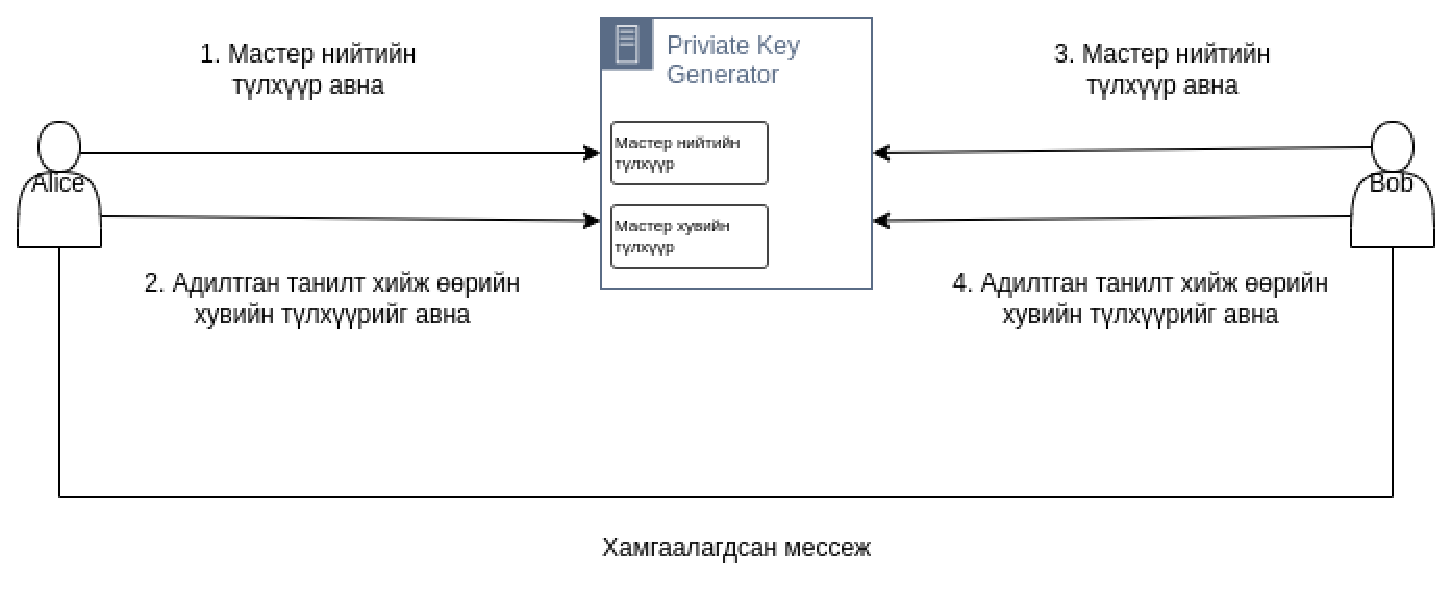
\includegraphics[scale=0.6]{Figures/IBE.eps}
\caption[IBE]{Танилтад суурилсан шифрлэлт}
\label{fig:IBE}
\end{figure}

IBE-дээр суурилсан алгоритмууд

\begin{itemize}
    \item Boneh–Franklin (BF-IBE)
    \item Sakai–Kasahara (SK-IBE)
    \item Boneh–Boyen (BB-IBE)
\end{itemize}

Давуу талууд

Сул талууд

\textbf{Шинж чанарт суурилсан шифрлэлэт (ABE)}

IBE-тэй ерөнхийдөө төстэй. Шинж чанаруудаар бүлэглэж зөвхөн нэг хэрлэгчийн түлхүүр ашиглахгүй олон хүн тайлах боломжтой.
Үндсэн хоёр төрөлтэй. Түлхүүр-Дүрэмийн шинж чанарт суурилсан шифрлэлт (KP-ABE) болон Шифртескт-Дүрэмийн шинж чанарт суурилсан шифрлэлт (CP-ABE).

ABE ерөнхий санаа нь сайн болов ч сул талуудтай.
\begin{itemize}
    \item Түлхүүр зохицуулалт
    \item Түлхүүр хадгалах
    \item Түлхүүр хүчингүй болгох
\end{itemize}

\textbf{KP-ABE}\\
Хэрэглэгч бүр 
\begin{figure}[ht]
    \centering
    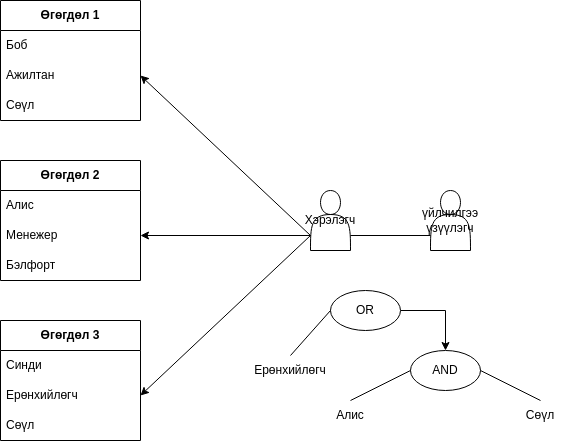
\includegraphics[scale=0.6]{Figures/kp-abe.drawio.png}
    \caption[IBE]{Танилтад суурилсан шифрлэлт}
\label{fig:kp-abe}
\end{figure}

\textbf{CP-ABE}\\

\begin{figure}[ht]
    \centering
    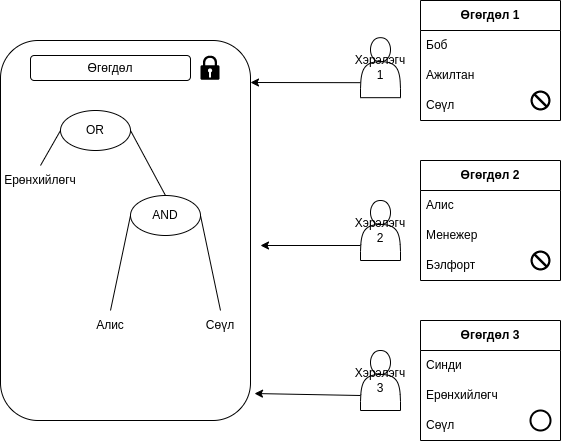
\includegraphics[scale=0.6]{Figures/cp-abe.drawio.png}
    \caption[IBE]{Танилтад суурилсан шифрлэлт}
    \label{fig:cp-abe}
\end{figure}

\textbf{Гомоморф шифрлэлт (HE)}

Энэ нь шифрлэгдсэн өгөгдлийг тайлахгүйгээр тооцоолол хийх боломжийг олгодог шифрлэлтийн төрөл юм.

\begin{itemize}
    \item Хэсэгчилсэн гомоморф шифрлэлт нь зөвхөн нэг төрлийн хаалга дэмждэг схемүүдийг хамардаг, жишээ нь нэмэх эсвэл үржүүлэх.
    \item Зарим төрлийн гомоморф шифрлэлтийн схемүүд нь хоёр төрлийн хаалгыг үнэлж чаддаг, гэхдээ зөвхөн хэлхээний дэд бүлэгт зориулагдсан.
    \item Түвшинтэй бүрэн гомоморф шифрлэлт нь хязгаарлагдмал (урьдчилан тодорхойлсон) гүнтэй олон төрлийн хаалганаас бүрдэх дурын хэлхээний үнэлгээг дэмждэг.
    \item Бүрэн гомоморф шифрлэлт (FHE) нь хязгааргүй гүнтэй олон төрлийн хаалганаас бүрдсэн дурын хэлхээг үнэлэх боломжийг олгодог бөгөөд гомоморф шифрлэлтийн хамгийн хүчтэй ойлголт юм.
\end{itemize}

%-------------------------------------------------------------------------------
%	SECTION 4
%-------------------------------------------------------------------------------

\section{Файл шифрлэх хадгалах}

Файлыг тэгш хэмт болон тэгч бус шифрэлэлтээр аль алингаар нь шифрлдэг. Тэгш хэмт шифрлэлт нь тэгш бус хэмт шифрлэлтээс хувьд хурдан боловч түлхүүр дамжуулах зэрэгт асуудал үүсдэг.

Файл системийн түвшинд шифрлэлтийг файлд суурилсан шифрлэлт (FBE) эсвэл файл/хавтас шифрлэлт гэдэг нэрлдэг дискний шифрлэлтийн нэг төрөл юм.

Файл системийн шифрлэлтийн төрөл
\begin{itemize}
    \item Криптограф файлын систем
    \item Ерөнхий зориулалт бүхий файлын шифрлэлт системүүд
\end{itemize}

Давуу талууд
\begin{itemize}
    \item Файлд суурилсан уян хатан түлхүүрийн удирдлага гэдэг нь файл бүрийг тусдаа түлхүүрээр шифрлэх боломжтой.
    \item Шифрлэгдсэн файлын тус тусд нь удирдах нь шифрлэгдсэн файлыг бүхэлд нь засаж өөрчлөхийн оронд зөвхөн өөрчлөгдсөн хэсгийг л өөрчлөх боломжтой.
    \item Хандалтын нийтийн түлрүүр ашиглах хянах боломжтой.
\end{itemize}

\textbf{Криптограф файлын систем}

Криптограф файлын системүүд нь шифрлэлт, аюулгүй байдлын үүднээс тусгайлан бүтээгдсэн (ерөнхий зориулалтын бус) файлын системүүд юм. Тэд ихэвчлэн мета өгөгдлийг оруулаад агуулсан бүх өгөгдлийг шифрлэдэг. Диск дээрх формат болон өөрийн блокийн хуваарилалт хийдэггүй одоо байгаа файлын системүүдийн дээр байрладаг.

\textbf{Ерөнхий зориулалт бүхий файлын шифрлэлт системүүд}

Криптограф файлын систем болон бүрэн дискний шифрлэлтээс ялгаатай нь файлын системийн түвшинд шифрлэлэт хийдэг ерөнхий зориулалтын файлын системүүд юм. Файлын нэр, хэмжээ, өөрчлөлтийн цагийн тэмдэг гэх мэт файлын системийн мета өгөгдлийг ихэвчлэн шифрлэдэггүй.

%-------------------------------------------------------------------------------
%	SECTION 5
%-------------------------------------------------------------------------------

\section{Бүлгийн Дүгнэлт}

Өгөгдөл хуваалцах болон өгөгдөлийн аюулгүй байдлын судалсан. Орчин үеийн шифрэлэлтийн схемүүдийн судлаж прокси дахин шифрлэх.
